% This example An LaTeX document showing how to use the l3proj class to
% write your report. Use pdflatex and bibtex to process the file, creating 
% a PDF file as output (there is no need to use dvips when using pdflatex).
% Modified 

% This dissertation was built upon base template provided.

\documentclass{l3proj}

\begin{document}

\title{Team I: ResDiary Restaurant Recommendation System}

\author{Vladimir Bardarski \\
        Paulius Dilkas \\
        Domantas Jurkus \\
        Edward Kalfov \\
        Josh O'brien \\
		Joseph O'Hagan}

\date{1 January 2000}

\maketitle

\begin{abstract}
The abstract shall go here! Here is some things to keep in mind while writing it.
\end{abstract}

\begin{itemize}
\item The abstract is likely the first substantive description of your work read by an examiner. View it as an opportunity to set accurate expectations.
\item The abstract is a summary of the whole thesis. It presents all the major elements of your work in a highly condensed form. (Write it having written the rest of the paper) The paper sets the abstract.
\item It must be capable of substituting for the whole paper when there is insufficient time and space for the full text.
\item Keep it short and snappy. 
\item The primary function of your thesis (and by extension your abstract) is not to tell readers what you did, it is to tell them what you discovered.
\item Approximately the last half of the abstract should be dedicated to summarizing and interpreting your results.
\item The most common error in abstracts is failure to present results.
\end{itemize}

% Comment out this line if you do not wish to give consent for your work to be distributed in electronic format.
% We hereby give consent - spread the knowledge - pending on result of project
\educationalconsent

\newpage

%==============================================================================
\section{Introduction}
% An introduction, explaining the purpose of the document, a very brief outline of the project and a summary of the structure of the rest of the document (approximately 1-2 pages).

The Professional Software Development (PSD3) course at The University of Glasgow requires students to engage with the practices and methodologies used in modern large-scale software engineering. The purpose of this dissertation is to document the development of the software project created as part of this course by Team I. 

The project was to build, over the course of several months, a restaurant recommendation engine for the Glasgow-based company ResDiary.
The goal was to deliver a system which could produce recommendations for restaurants to a user, that could be integrated into their existing systems at a later date. 

Our team consisted of six third-year Computing Science students. Within the group there was a broad array of skills, interests and experience - with two members actively working as software professionals, and another having participated in an internship. For some members, however, this was a first opportunity to interact with a real client. 

In this document we outline, in detail, the entire process: from the initial requirements gathering with our customer, through to final system delivery. 

In section \ref{sec:background} we present the background to the project, the motivations of the customer and how we arrived at the agreed deliverables.

%this will surely be expanded to enumerate each separate section better I would like to discuss in detail the practices, issue-tracking, the team work/team load - Josh etc.

In subsequent sections \ref{sec:alice} through Section \ref{sec:reflections} we explore the challenges we faced through development and the steps we took to resolve them, explore the impact of team dynamics on the outcome and reflect on what we have learned from the experience. We also explain how we applied the good development practices learned in PSD3. In particular we highlight the role of version control, agile development and issue tracking.

\newpage

%==============================================================================
\section{Case Study Background}
\label{sec:background}
% A description of the case study background and context. This should include a description of the project customer (what was the nature of the organisation you were working for), their objectives for the project, and a summary of what was actually achieved. Where appropriate, this section should also make reference to similar related projects in order to make the context clear (approximately 4-5 pages).

\subsection{Customer}
\label{customer}
% The customer organisation and background.

% -- Old copy --
% ResDiary is a Glasgow based online restruant reservation system which was founded in 2006. They are a commerical organisation whose service provides a commission-free online reservation system. Their aim is to provide a booking platform and table management system that is comprehensive and easy to use by both the hospitality industry and their guests. 
% For the duration of the project ResDiary senior software engineer's Adam Connelly and Ian Strachan served as both the customer and contact for the project. 
% --------------

ResDiary is a Glasgow based online restruant reservation system which was founded in 2006. They are a commerical organisation whose service aims to provide a booking platform and table management system that is comprehensive and easy to use by both the hospitality industry and their guests.
For the duration of the project ResDiary senior software engineer's Adam Connelly and Ian Strachan were the representatives of ResDairy for the project.
Primarily we interacted with Ian Strachan, as he was whom we initially met with during the requirements elicitation meeting and contacted to request additional data resources provided by ResDairy throughout the duration of the project.
Both Ian Strachan and Adam Conlley were in attendance at each iteration meeting, unless conflicting commitments rendered then unable to attend, and both provided useful feedback and insight whilst discussing some of the design decisions we were making and answering our queries throughout the duration of the project.

\subsection{Initial Objectives And Rationale}
\label{initobjectives}
% The rationale and initial objectives for the project.

The initial customer requirements elicitation meeting was lead by ResDiary senior software engineer Ian Strachan. 

- WIP Initial Meeting Notes : Justification / Pitch of Project -
At the meeting an overview was given of the ResDiary business and service. 
They explained how their current portal allows diners to search for restaurants and available tables for dining but this requires users to select a specific date and general location. 
They wish to improve restaurant discovery on their service and hope a restraurant recommendation engine could be created and at a later date integrated into the site.
The goal of the project is to create a recommendation engine that accurately suggests places to eat based on previous restaurants visited by the user and other users with similar dining habits.
The recommendations must be in close proximity to restaurants the user typically visits. A user who eats out in Glasgow should have recommendations to restraunts in Glasgow.
They believed that none of their competition have a similar feature and feel it would give them the edge in the restaurant booking portal world.
They wished to explore a potential use for their collection of big data which is currently not being used. 
- - - -  

- WIP NOTES : 
From the offset we faced a decision to either use Python or C# primarily for development. ResDiary uses C# for their development but one of the team members with some experience working on recommendation systems and big data sets felt that Python was better suited at least initially for the project. 
- - - - 

- WIP NOTES (SHOULD BE WORKED IN SOMEHOW) -
Intially it was unsure of how the final product would be used by ResDiary. 
Both integration into their existing site and creation of an API to access the application were proposed during the initial stages. 
Ultimately the customers mindset shifted and wished to use the project as a proof of concept and learning tool for their own use.
They wished to be given the end product so they could then assess its usefulness and quality and investigate if integration of a similar service into their own site would be beneficial.
They were also unaware of how to build such a service and so would like to sort of reverse engineer the project to understand how a similar system could be built into their existing service.
The team also currently has a large quantity of big data they are currently not ultising for anything and so would like to use the project as a proof of concept for ultilising their big data resource for additional projects and services down the line.

\subsection{Delivered Software}
\label{finsoftware}
% Information on the final software that was delivered to the customer.

\newpage

%==============================================================================
\section{Alice}
\label{sec:alice}

ALICE \cite{alice} was beginning to get very tired of sitting by her sister
on the bank and of having nothing to do: once or twice she had peeped into
the book her sister was reading, but it had no pictures or conversations in
it, ``and what is the use of a book,'' thought Alice, ``without pictures or
conversations?'

\begin{figure}
\begin{center}
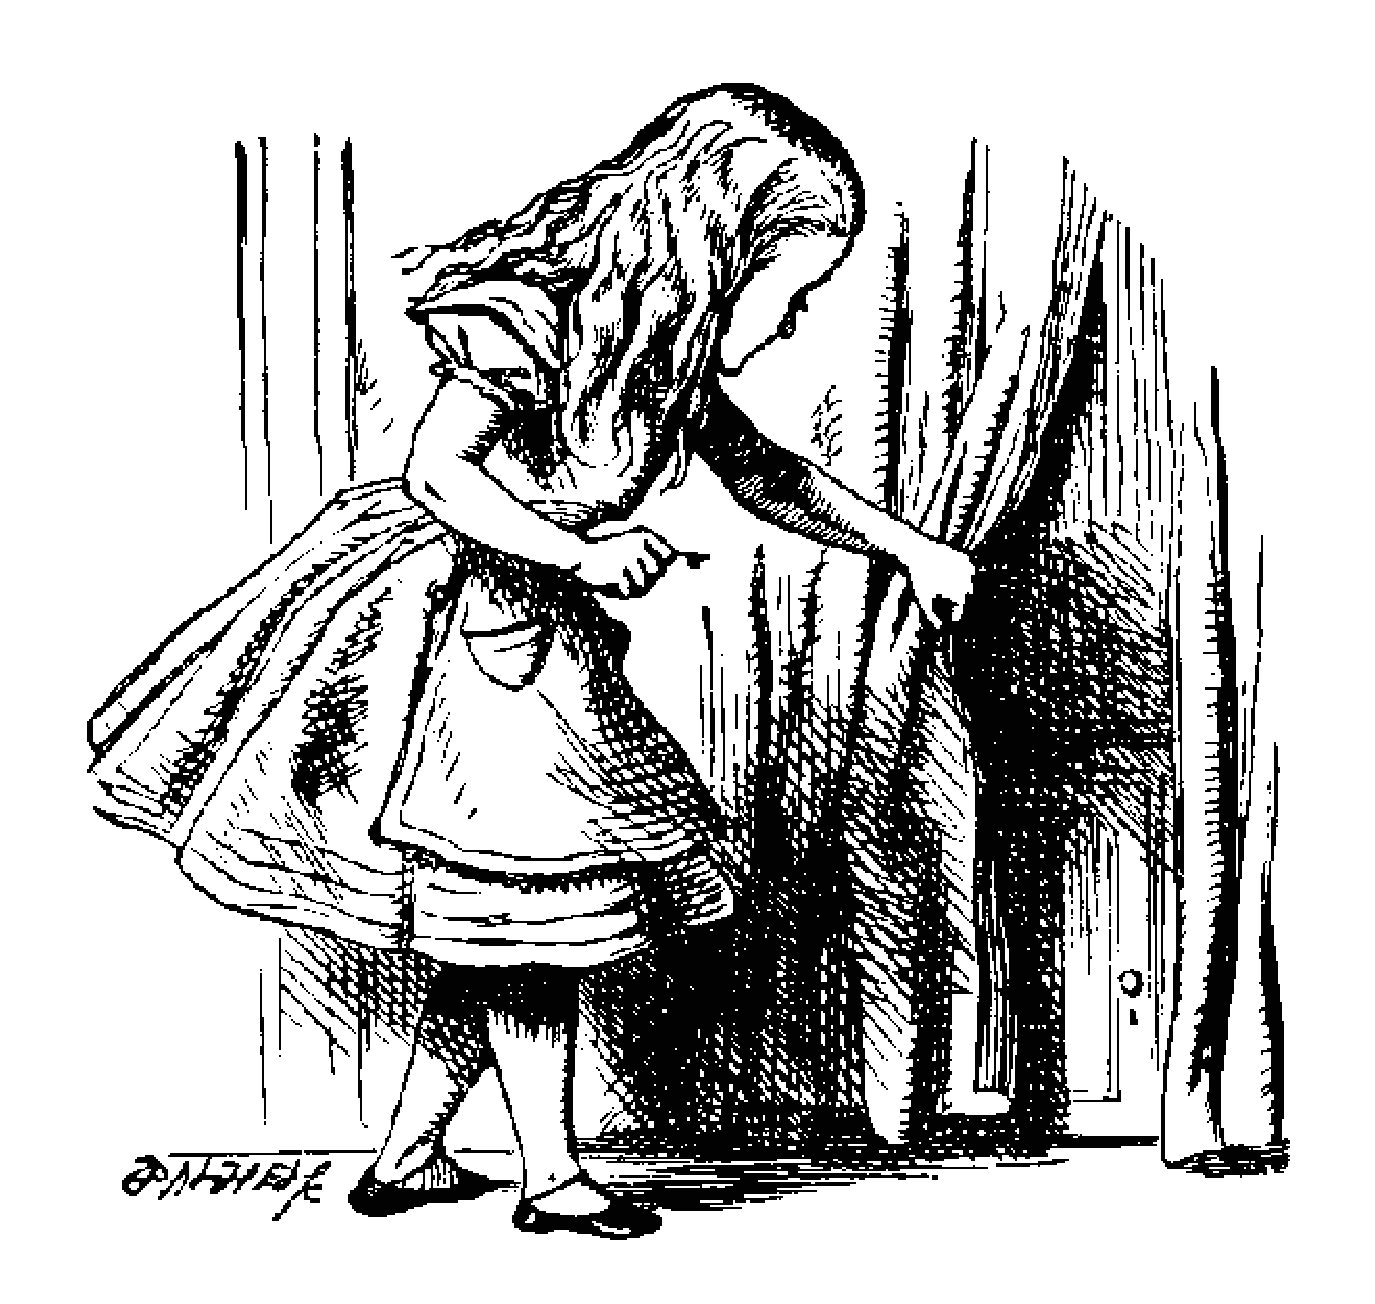
\includegraphics[width=7cm]{figures/alice}
\end{center}
\caption{Behind it was a little door}
\label{fig:alice}
\end{figure}

Alice opened the door (see Figure \ref{fig:alice}) and found that it
led into a small passage, not much larger than a rat-hole: she knelt
down and looked along the passage into the loveliest garden you ever
saw. How she longed to get out of that dark hall, and wander about
among those beds of bright flowers and those cool fountains, but she
could not even get her head through the doorway; ``and even if my head
would go through,'' thought poor Alice, ``it would be of very little
use without my shoulders. Oh, how I wish I could shut up like a
telescope! I think I could, if I only knew how to begin.'' For, you
see, so many out-of-the- way things had happened lately, that Alice
had begun to think that very few things indeed were really impossible.

%==============================================================================

\section{Choice of Colours}
\label{design}

The following diagrams (especially figure \ref{fig:alice}) illustrate the
process...

%==============================================================================
\section{Managing Dress Sense}
\label{managing}

In this chapter, we describe how the implemented the system.

% - - - - - - - - - - - - - - - - - - - - - - - - - - - - - - - - - - - - - - -
\section{Reflections}
\label{sec:reflections}
% Several sections that reflect on your experiences during the team project. Each section should discuss one theme, characterised by incidents or events that occurred during the team course of the project from which you learned (approximately 12-15 pages).

%------------------------------------------------------------------------------
\section{Conclusions}
\label{sec:conclusions}
% A conclusion that draws general and wider lessons from the case study (approximately 1-2 pages)

Explain the wider lessons that you learned about software engineering,
based on the specific issues discussed in previous sections.  Reflect
on the extent to which these lessons could be generalised to other
types of software project.  Relate the wider lessons to others
reported in case studies in the software engineering literature.

%==============================================================================
\bibliographystyle{plain}
\bibliography{dissertation}
\end{document}
